\documentclass[a4paper,12pt]{article}
%%%%%%%%%%%%%%%%%%%%%%%%%%%%%%%%%%%%%%%%%%%%%%%%%%%%%%%%%%%%%%%%%%%%%%%%%%%%%%%%%%%%%%%%%%%%%%%%%%%%%%%%%%%%%%%%%%%%%%%%%%%%%%%%%%%%%%%%%%%%%%%%%%%%%%%%%%%%%%%%%%%%%%%%%%%%%%%%%%%%%%%%%%%%%%%%%%%%%%%%%%%%%%%%%%%%%%%%%%%%%%%%%%%%%%%%%%%%%%%%%%%%%%%%%%%%
\usepackage{eurosym}
\usepackage{vmargin}
\usepackage{amsmath}
\usepackage{graphics}
\usepackage{epsfig}
\usepackage{enumerate}
\usepackage{multicol}
\usepackage{subfigure}
\usepackage{fancyhdr}
\usepackage{listings}
\usepackage{framed}
\usepackage{graphicx}
\usepackage{amsmath}
\usepackage{chngpage}
%\usepackage{bigints}

\usepackage{vmargin}
% left top textwidth textheight headheight
% headsep footheight footskip
\setmargins{2.0cm}{2.5cm}{16 cm}{22cm}{0.5cm}{0cm}{1cm}{1cm}
\renewcommand{\baselinestretch}{1.3}

\setcounter{MaxMatrixCols}{10}

\begin{document}
\large
\noindent Consider the n = 30 independent and identically distributed observations
$( y_1 , y_2 , \ldots, y_n )$ given below from a random variable Y with probability distribution
\[\theta y e –\theta
function f ( y, \theta) =
.
y! \]


You can enter the y values into R by using:


\begin{framed}\begin{verbatim}

y = c(5,5,6,2,4,10,2,5,5,2,5,3,7,     4,4,5,4,6,7,2,8,4,6,4,3,6,
      6,6,5,7)

\end{verbatim}\end{framed}


By assuming a prior distribution proportional to $e^{–a\theta}$ , we can show that the posterior
distribution of $\theta$ is:
\[
\sum^{n}_{i=1}y
f (\theta | y 1 , y 2 ,..., y n ) \propto \theta i=1 i e –(n + \alpha) \theta
\]
We can observe that the posterior distribution of $\theta$ is Gamma with parameters
n
∑ i=1 y i – 1 and n + a.

%%%%%%%%%%%%%%%%%%%%%%%%%%
\newpage 
Plot the posterior probability density function of $\theta$ for values of $\theta$ in
the interval [3.2, 6.8] and assuming a = 0.01.
		
[Hint: the range of values of $\theta$ can be obtained in R by
seq(3.2, 6.8, by = 0.01).]
(b)
Carry out a simulation of N = 5,000 posterior samples for the
parameter $\theta$.

(i) (a)
(ii) Plot the histogram of the posterior distribution of $\theta$.




Q2


\begin{framed}\begin{verbatim}
y = c (5, 5, 6, 2, 4, 10, 2, 5, 5, 2, 5, 3, 7, 4, 4, 5, 4, 6,
7, 2, 8, 4, 6, 4, 3, 6, 6, 6, 5, 7)

## plot the posterior pdf of theta
theta = seq(3.2, 6.8, by = 0.01)
\end{verbatim}\end{framed}

%%%%%%%%%%%%%%%%%%%%%%%%%%%
\newpage 

\begin{framed}\begin{verbatim}
plot(theta, dgamma(theta, sum(y)-1, length(y) + 0.01), 
     ylab = "Density", type = "l")
\end{verbatim}\end{framed}


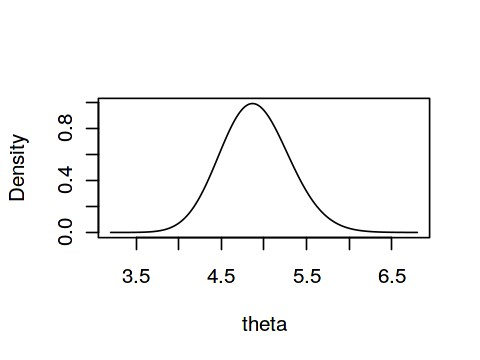
\includegraphics[]{00-A1/images/Exercise_2_A.jpeg}


The posterior samples are
\end{verbatim}\end{framed}{r}
x = rgamma(5000, sum(y)-1, 30 + 0.01)
\end{verbatim}\end{framed}



%%%%%%%%%%%%%%%%%%%%%%%%%%%%%%%%%%%%%%
\newpage 
\subsection*{Exercise 2}


We can plot the histogram using



\begin{framed}
\begin{verbatim}
x = rgamma(5000, sum(y)-1, 30 + 0.01)
\end{verbatim}
\end{framed}


\begin{framed}
\begin{verbatim}
hist(x, main="Posterior distribution of theta",xlab="theta")
\end{verbatim}
\end{framed}

%%%%%%%%%%%%%%%%%%%%%%%%%%%%%%%%%%%%%%%%%%%%%%%%%%%%%%
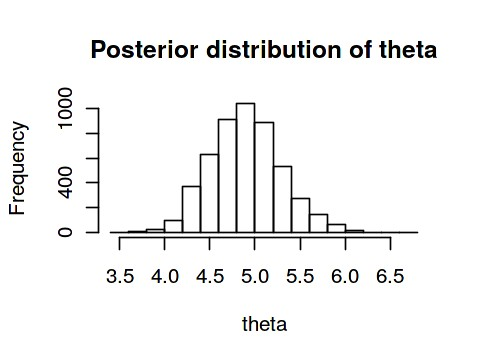
\includegraphics[]{00-A1/images/Exercise_2_B.jpeg}



\begin{framed}\begin{verbatim}
\end{verbatim}\end{framed}
[1]
Posterior distribution of
3.5
4.0
4.5
5.0
5.5
6.0
6.5
theta
%%%%%%%%%%%%%%%%%%%%%%%%%%%%%%%%%%%%%%
\newpage 
\subsection*{Exercise 3}

\noindent Calculate the mean, median and standard deviation of the posterior distribution
of $\theta$.

\begin{framed}
\begin{verbatim}
mean(x)
# 5.003996 

median(x)
# 4.997373

sd(x)
# 0.4117624 
\end{verbatim}
\end{framed}

Two possible values for the true value of parameter $\theta$ are $\theta$ =15 and $\theta$ = 5.


15 is quite far away from the range of samples obtained for the posterior distribution
of $\theta$.
On the other hand 5 is more likely to be the true value.


%%%%%%%%%%%%%%%%%%%%%%%%%%%%%%%%%%%%%%
\newpage 
\subsection*{Exercise 5}

Comment on these two values based on the posterior distribution of $\theta$ plotted
in part (ii) and summarised in part (iii).



15 is very unlikely to be the case if there is no calculation error.

5 fits well within the distribution and the values of the mean and the median are very close to it.

%%%%%%%%%%%%%%%%%%%%%%%%%%%%%%%%%%%%
\newpage
BLANK
\newpage
%%--- #### R
Parts (i), (ii) and (iii) were generally well answered. A common error was to use sum(y-1)
instead of sum(y)-1 in the computations. 

In part (iii) a number of candidates provided the
answers using the theoretical results based on the given posterior distribution – this was
given full credit. Note that displaying the plots is required for full marks. 

Note that the parameter of the gamma distribution given as ∑ nnii−1 yy ii − 1 in the preamble of
the question is theoretically incorrect and should have been ∑ nnii−1 yy ii + 1 . 


The error did not
affect the remainder of the question and the required answer, as the candidates were
explicitly asked to work with the ∑ nnii−1 yy ii − 1 quantity as given in the question. The
examiners did not find evidence of this error having a negative impact on candidates’
performance.

\end{document}
